\chapter{Requirements und Use Cases}

\section{Systemebene}

Die Anforderungen aus der Aufgabenstellung sind nicht vollständig. Die
Struktur der nachfolgenden Kapitel soll sie bei der Strukturierung der
Analyse unterstützen. Dokumentieren Sie die Ergebnisse der Analysen
entsprechend.

\subsection{Stakeholder}

Ermitteln sie die Stakeholder für das Projekt und listen sie diese hier
auf.

\subsection{Anforderungen}

In der Aufgabenstellung sind Anforderungen an das System gestellt.
Arbeiten sie diese hier auf und ergänzen sie diese entsprechend der
Absprachen mit dem Betreuer. Achten sie auf die entsprechende
Atribuierung. 
Berücksichtigen sie auch mögliche Fehlbedienungen und Fehlverhalten des
Systems.

% TODO: Correctly typeset the following Requirement tables
% FIXME: Set column width according to pagewidth
% FIXME: Define column width globally
Requirements:\\\\
\begin{tabular}{|p{3 cm} |p{9 cm}|}
	\hline
	REQ -- 01 & Laufband starten  \\
	\hline
\end{tabular}
	Die Software soll das Laufband starten sobald ein Werkst{\"u}ck auf den Anfang gelegt wird.\\
	\\
\begin{tabular}{|p{3 cm} |p{9 cm}|}
	\hline
	REQ -- 02 & Werkst{\"u}cke sortieren\\
	\hline
\end{tabular}
	Die Software sortiert Werkst{\"u}cke laut dem vorgegebenen Schema: Bohrung oben ohne Metalleinsatz, Bohrung oben ohne Metalleinsatz, Bohrung oben mit Metalleinsatz. \\\\
\begin{tabular}{|p{3 cm} |p{9 cm}|}
	\hline
	REQ -- 03 & Durchlaufzeiten messen \\
	\hline
\end{tabular}
Die Software misst die Durchlaufzeiten der  Werkst{\"u}cke, damit das Hinzuf{\"u}gen und verloren gehen von  Werkst{\"u}cken registriert wird.\\\\
\begin{tabular}{|p{3 cm} |p{9 cm}|}
	\hline
	REQ -- 04 & Weichen steuern \\
	\hline
\end{tabular}
Die Software kann die Weichen {\"o}ffnen und so die Werkst{\"u}cke sortieren.\\\\
\begin{tabular}{|p{3 cm} |p{9 cm}|}
	\hline
	REQ -- 05 & B{\"a}nder stoppen\\
	\hline
\end{tabular}
Die Software stoppt die Laufb{\"a}nder, wenn siche keine Werkst{\"u}cke darauf befinden.\\\\
\begin{tabular}{|p{3 cm} |p{9 cm}|}
	\hline
	REQ -- 06 & Fehler signalisieren \\
	\hline
\end{tabular}
Die Software gibt bei Fehlern Fehlermeldungen auf der Konsole aus und signalisiert einen Fehler zus{\"a}tzlich durch die Rote Ampel.\\\\
\begin{tabular}{|p{3 cm} |p{9 cm}|}
	\hline
	REQ -- 07 &Werkst{\"u}cke erkennen \\
	\hline
\end{tabular}
Die Software erkennt verschiedene Typen von Werkst{\"u}cken und gibt die Typkennung auf der Konsole aus sobald sie bekannt ist.\\\\
\begin{tabular}{|p{3 cm} |p{9 cm}|}
	\hline
	REQ -- 08 &Kommunikation \\
	\hline
\end{tabular}
Die Software erm{\"o}glicht Kommunikation zwischen zwei Laufb{\"a}ndern.\\\\
\begin{tabular}{|p{3 cm} |p{9 cm}|}
	\hline
	REQ -- 09 & Volle Rutschen \\
	\hline
\end{tabular}
Die Software erkennt wenn die Rutschen zum Aussortieren voll sind und Sortiert die Werkst{\"u}cke dann auf dem anderen Band.\\\\
\begin{tabular}{|p{3 cm} |p{9 cm}|}
	\hline
	REQ -- 10 &Mehrerer Werkst{\"u}cke \\
	\hline
\end{tabular}
Die Software kann mehrere Werkst{\"u}cke auf dem ersten Laufband bearbeiten und sorgt daf{\"u}r, dass sich nur ein einziges Werkst{\"u}ck zur Zeit auf dem zweiten Laufband befindet.\\\\
\begin{tabular}{|p{3 cm} |p{9 cm}|}
	\hline
	REQ -- 11 &Sortierte Werkst{\"u}cke \\
	\hline
\end{tabular}
Die Software gibt f{\"u}r Werkst{\"u}cke die das Ende des zweiten Laufbandes erreichen, die ID, den Typ, H{\"o}henmesswert 1 und H{\"o}henmesswert 2 auf der Konsole aus.\\\\
\begin{tabular}{|p{3 cm} |p{9 cm}|}
	\hline
	REQ -- 12 &Bedientaster \\
	\hline
\end{tabular}
Die Software kann mit den Bedientastern Ein/Aus geschaltet werden und verf{\"ugt} {\"u}ber eine E-Stop Funktion, die die komplette Anlage zum Stillstand bringt.\\\\
\begin{tabular}{|p{3 cm} |p{9 cm}|}
	\hline
	REQ -- 13 &Geschwindigkeit anpassen \\
	\hline
\end{tabular}
Die Software passt die Geschwindigkeit der Laufb{\"a}nder so an das sie langsam durch die H{\"o}henmessung fahren.\\\\
\subsection{Systemkontext}

Die Sicht, aus der die Use Cases verfasst wurden, geht aus
\autoref{fig:systemcontextdiagram} hervor.

\begin{figure}
    \centering
    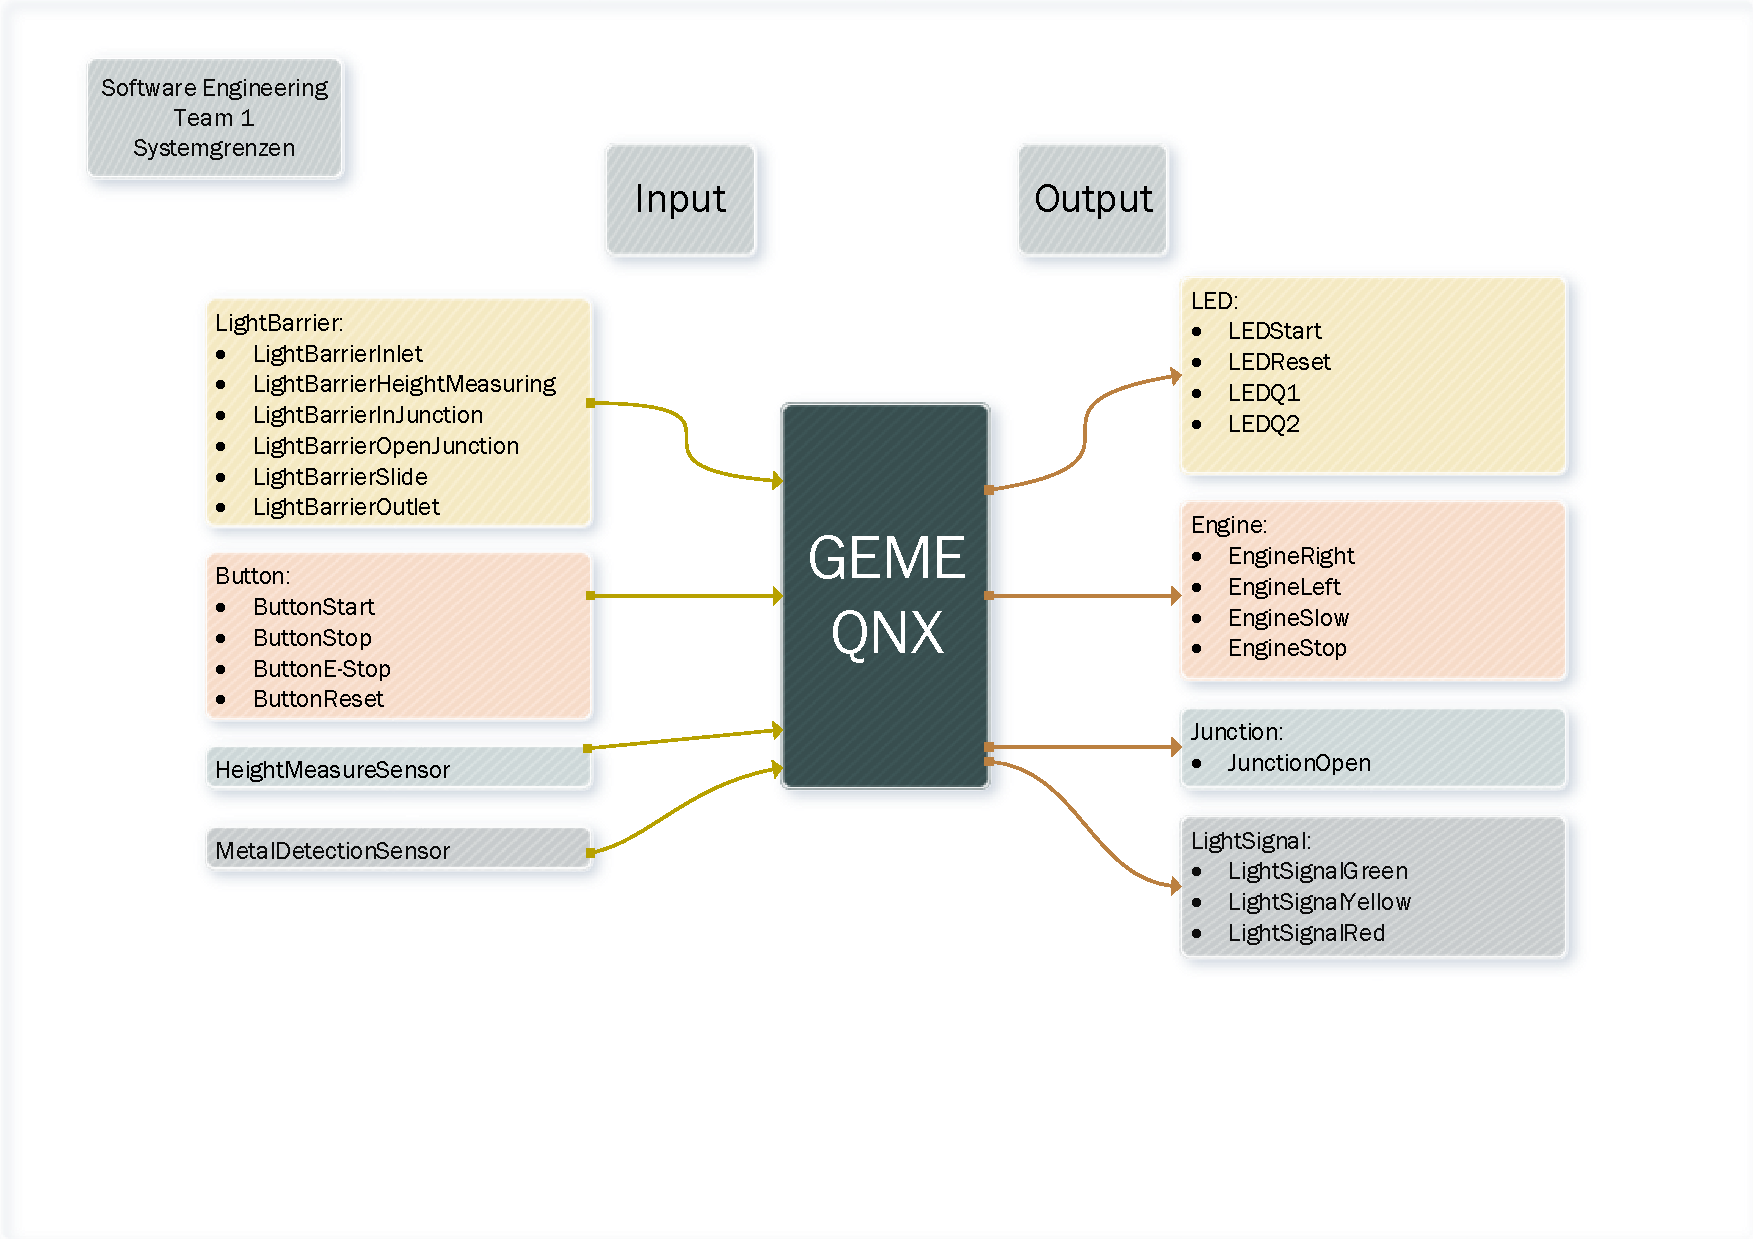
\includegraphics[width=\textwidth]{figures/systemcontext.pdf}
    \caption{Systemkontextdiagramm}
    \label{fig:systemcontextdiagram}
\end{figure}

\subsection{Use Cases}

Dokumentieren sie hier, welche Use Cases sie auf der Systemebene
implementieren müssen. Die Test Cases sollen später zu den Use Cases
konsistent sein.

\begin{tabular}{|p{3 cm} |p{9 cm}|}
	\hline
	ID & UC-01 \\
	\hline
	Name & Werkst{\"u}ck sortieren\\
	\hline
	Autoren & Dennis Kochinky\\
	\hline
	Priorit{\"a}t & Hoch\\
	\hline
	Verantwortliche & ESEP-Team 1.2\\
	\hline
	Akteure & Band, Lichtschranken, Weichen, Steuerungssoftware, User\\
	\hline
	Kurzbeschreibung & Ein Werkst{\"u}ck wird auf das Band, vermessen und  einsortiert.\\
	\hline
	Ausl{\"o}sendes Ereignis & Werkst{\"u}ck wird auf das erste Laufband gelegt.\\
	\hline
	Vorbedingung & Anfang des ersten Bandes ist frei, Anlage ist Betriebsbereit.\\
	\hline
	Nachbedingung & Werkst{\"u}ck hat Ende des zweiten Bandes erreicht.\\
	\hline
	Ergebnis & Werkst{\"u}ck einsortiert\\
	\hline
	Hauptszenario & \begin{enumerate}
	\item Werkst{\"u}ck wird auf Band 1 gelegt.  
	\item Die Software erkennt Unterbrechung der Lichtschranke und startet das Band.	
	\item Werkst{\"u}ck erreicht im vorgegeben Zeitfenster die H{\"o}henmessung und wird analysiert. 
	\item Weiche wird ge{\"o}ffnet.
	\item Werkst{\"u}ck wird auf Band 2 {\"u}bergeben.
	\item Erfassung, H{\"o}henmessung des Werkst{\"u}ckes und {\"o}ffnen der Weiche auf Band 2. 
	\item Werkst{\"u}ck hat das Ende von Band 2 erreicht.
	\end{enumerate}
           \\
	\hline
	Alternativszenario 1 & 4a) Das Werkst{\"u}ck ist zu flach, die Weiche bleibt geschlossen und das Werkst{\"u}ck wird auf die Rutsche geleitet.\\
	\hline
	Alternativszenario 2 & 6a) Werkst{\"u}ck wird f{\"u}r die Sortierung nicht gebraucht, die Weiche auf Band 2 bleibt geschlossen und das Werkst{\"u}ck wird auf Rutsche 2 aussortiert. \\
	\hline
	Fehlerszenario &  3a) Werkst{\"u}ck ist zu schnell (ein weiteres Werkst{\"u}ck wurde zwischendurch aufs Band gelegt) oder Werkst{\"u}ck ist zu langsam ( ein Werkst{\"u}ck wurde entfernt), das Band wird gestoppt.\\

	\hline
	
	
\end{tabular}

\begin{tabular}{|p{3 cm} |p{9 cm}|}
	\hline
	ID & UC-02 \\
	\hline
	Name &  Rutsche voll.\\
	\hline
	Autoren & Dennis Kochinky\\
	\hline
	Priorit{\"a}t &  Mittel\\
	\hline
	Verantwortliche & ESEP-Team 1.2\\
	\hline
	Akteure & Band, Lichtschranken, Weichen, Steuerungssoftware, User\\
	\hline
	Kurzbeschreibung & Die Software erkennt, dass eine der Rutschen voll ist und setzt das Aussortieren auf dem anderen Band mit  		freier Rutsche fort\\
	\hline
	Ausl{\"o}sendes Ereignis & Die Lichtschranke an der Rutsche ist dauerhaft unterbrochen.\\
	\hline
	Vorbedingung & Werkst{\"u}cke sind auf dem Band. \\
	\hline
	Nachbedingung & Sortierung wird auf dem Band mit freier Rutsche fortgesetzt.\\
	\hline
	Ergebnis & Dem User wird die volle Rutsche signalisiert und Sortierung läuft weiter. \\
	\hline
	Hauptszenario & \begin{enumerate}
	\item Ein Werkst{\"u}ck wird auf Band 1 gelegt.  
	\item Die Software erkennt, dass die Rutsche voll ist und signalisiert dies durch die gelbe Ampel.	
	\item Die Weiche wird ge{\"o}ffnet.
	\item Werkst{\"u}ck erreicht Ende von Band 1 und wird auf Band 2 {\"u}bergeben.
	\item Sortierung wie in UC-01.
	\end{enumerate}
           \\
	\hline
	Alternativszenario & \begin{itemize} 
	\item [2.1a] Beide B{\"a}nder melden Rutsche voll. 
	\item [2.1b] Band wird gestoppt und Fehler signalisiert.
	\end{itemize}
	\\
	\hline
\end{tabular}
	
\begin{tabular}{|p{3 cm} |p{9 cm}|}
	\hline
	ID & UC-03 \\
	\hline
	Name & Kalibrierung\\
	\hline
	Autoren & Dennis Kochinky\\
	\hline
	Priorit{\"a}t & Hoch\\
	\hline
	Verantwortliche & ESEP-Team 1.2\\
	\hline
	Akteure & Band, Lichtschranken, Weichen, Steuerungssoftware, User\\
	\hline
	Kurzbeschreibung & System wird nach dem einschalten kalibriert, dazu wird ein Werkst{\"u}ck  auf das Band gelegt.\\
	\hline
	Ausl{\"o}sendes Ereignis & System wird eingeschaltet und ein Werkst{\"u}ck wird vom User auf das erste Band gelegt.\\
	\hline
	Vorbedingung & Das System ist im Startzustand.\\
	\hline
	Nachbedingung & Alle Sensoren und Aktore funktionieren.\\
	\hline
	Ergebnis & Werkst{\"u}ck ist am Ende von Band 2 angekommen.\\
	\hline
	Hauptszenario & \begin{enumerate}
	\item Das System wird eingeschaltet.
	\item Ein Werkst{\"u}ck wird auf Band 1 gelegt.  
	\item Die Software erkennt Unterbrechung der Lichtschranke und startet das Band (Timer).	
	\item Werkst{\"u}ck erreicht die H{\"o}henmessung, Bandgeschwindigkeit wird verlangsamt.
	\item Die Weiche wird ge{\"o}ffnet.
	\item Werkst{\"u}ck erreicht Ende von Band 1 und wird auf Band 2 {\"u}bergeben.
	\item Daten werden auf der Konsole ausgegeben.
	\item Weiter mit Band 2.
	\end{enumerate}
           \\
	\hline
	Fehlerszenario & Band oder Weiche kann nicht angesteuert werden, Werkst{\"u}ck landet auf Rutsche. \\
	\hline
\end{tabular}

\begin{tabular}{|p{3 cm} |p{9 cm}|}
	\hline
	ID & UC-04 \\
	\hline
	Name & E-Stopp\\
	\hline
	Autoren & Dennis Kochinky\\
	\hline
	Priorit{\"a}t & Mittel\\
	\hline
	Verantwortliche & ESEP-Team 1.2\\
	\hline
	Akteure & E-Stopp-Taster, Band, Weichen, User\\
	\hline
	Kurzbeschreibung &  Bet{\"a}tigung des E-Stopp-Tasters sorgt f{\"u}r Abschaltung der B{\"a}nder.\\
	\hline
	Ausl{\"o}sendes Ereignis & E-Stopp-Taster wird vom User gedr{\"u}ckt\\
	\hline
	Vorbedingung & Das System in Betrieb.\\
	\hline
	Nachbedingung & B{\"a}nder stehen still und Weichen sind geschlossen.\\
	\hline
	Ergebnis & Komplette Anlage steht still.\\
	\hline
	Hauptszenario & \begin{enumerate}
	\item E-Stopp-Taster wird vom User gedr{\"u}ckt.
	\item Die B{\"a}nder werden gestoppt.
	\item Die Weichen werden geschlossen.
	\item Die Ampel wird ausgeschaltet.
	\item Warten auf Reset.
	\end{enumerate}
           \\
	\hline

\end{tabular}

\section{Systemanalyse}
Ihr technisches System hat aus Sicht der Software bestimmte
Eigenschaften. Was muss man für die Entwicklung der Software in
Struktur, Schnittstellen, Verhalten und an Besonderheiten wissen? Wählen
sie eine Kapitelstruktur, die am besten zur Dokumentation ihrer
Ergebnisse geeignet ist.

\section{Softwareebene}

Sie sollen Software für die Steuerung des technischen Systems erstellen.
Aus den Anforderungen auf der Systemebene und der Systemanalyse ergeben
sich Anforderungen für Ihre Software. Insbesondere wird sich die
Software der beiden Anlagenteile in einigen Punkten unterscheiden.
Dokumentieren sie hier die Anforderungen, die sich speziell für die
Software ergeben haben.

\subsection{Systemkontex}

Wie sieht der Kontext Ihrer Software aus? Wie erfolgt die Kommunikation
mit Nachbarsystemen? Liste der ein- und ausgehenden Signale/Nachrichten.

\subsection{Anforderungen}

Welche wesentlichen Anforderungen ergeben sich aus den
Systemanforderungen für ihre Software? Achten sie auf die entsprechende
Atribuierung. Berücksichtigen sie auch mögliche Fehlbedienungen und
Fehlverhalten des Systems.
